\documentclass{beamer}
%\documentclass[notes]{beamer}

\usetheme{Warsaw}

\usepackage{inputenc}
\usepackage{graphicx}

\title{Foundations of Empirical Memory Consistency Testing}
\subtitle{Jake Kirkham, Tyler Sorenson, Esin Tureci, Margaret Martonosi}

\author{Presented by \\ Akshay Gopalakrishnan}
\institute{McGill University}

\begin{document}
    
    \begin{frame}

        \titlepage

    \end{frame}

    %Introduction
    \begin{frame}{Introduction}

        \begin{itemize}
            \item Testing semantics of Shared Memory Consistency w.r.t. their parent Hardware.
            \item Testing done using various parameters forcing the hardware to proc Relaxed Behaviors.
            \item Testing done on the OpenCL memory consistency model running on various GPU/CPU bases.
            \item Bugs detected hint towards compiler bugs (in this paper that of Intel x86)/ hardware bugs hinting towards misrepresentation of the behaviors of Hardware..  
        \end{itemize}

    \end{frame}

    %Memory consistency model
    \begin{frame}{Memory Consistency Models}

        \begin{itemize}
            \item Semantics defining the possible values a memory read can give in execution of concurrent programs. 
            \item Required to write concurrent programs using shared memory concurrency.
            \item Our intuitive reasoning of concurrent programs rely on Sequential Consistency. 
        \end{itemize}
        
        \textit{The outcome of an execution of a program is equivalent to the same program running in a uniprocessor setting (interleaving semantics).}

    \end{frame}

    %The need for testing 
    \begin{frame}{Why Empirical Testing as opposed to Formal Proofs?}

        \begin{itemize}
            \item Formal proofs regarding memory consistency (compiler mappings and memory model implementation) are done manually. 
            \item Compiler technology is ever evolving, and manual efforts needed to account for new parts of languages (which influence concurrent programs).
            \item Hardware proofs (checking implementation of memory model w.r.t. hardware behaviors) have been applied only to small systems or toy models.
            \item Existing proofs have sometimes also been shown to be incorrect (mainly through counter examples).
            \item Empirical testing has shown promise to identify bugs in compilers and microarchitectural features.
            \item Litmus tests run for a million iterations gives much confidence towards validation of the system w.r.t. semantics defined. 
        \end{itemize}

        %Elicit the importance of empirical testing over writing formal proofs.
    \end{frame}

    %Deficiencies of previous testing methods
    \begin{frame}{Previous Testing Framework Deficiencies}

        \begin{itemize}
            \item Reproducibility - Often difficult to reproduce the same set of bugs in the same setting (require more fine grained setting).
            \item False Negatives - Does not guarantee lack of bugs (its confidence can be enhanced using some measures of probability).
            \item Redundant testing time - Often over testing is done (this can be managed using probabilistic guarantees) .
        \end{itemize}

    \end{frame}

    %Parameterizing test bed
    \begin{frame}{Proposed Testing framework with Parameters}

        %List the parameters that will be used.
        \begin{itemize}
            \item Stressing and Testing.
            \item Barrier and Occupancy.
            \item Id Shuffling and Oversubscription.
        \end{itemize} 

    \end{frame}

    %Parameter 1
    \begin{frame}{Memory Parameters: Stressing and Testing Parameter}

        \begin{itemize}
            \item Memory is divided into two parts : Stressing and Testing.
            \item Testing memory - Memory using which our target program operates/ executes.
            \item Stressing memory - Memory not touched by the target program.
        \end{itemize}
        
        It is called stressing memory because for testing, we would employ programs to heavily use the stressing memory section.
        This would influence the role of caches in the execution. 
        Also, it would give us insight on how other physical parameters (temperature, power consumption, etc.) would affect.

    \end{frame}

    %Parameter 2
    \begin{frame}{Concurrency Parameters: Barrier and Occupancy}

        \begin{itemize}
            \item In any multi-core experiment, it could be that each thread is spawned for execution or assigned to cores in an uneven manner.
            \item It could even result in the whole execution being sequential in time. 
            \item This would prevent any relaxed behaviors from being observed. 
            \item Hence, a barrier is used to ensure uniform spawning of threads for them to possibly exhibit relaxed behaviors.
        \end{itemize}
        
        %NOTE: NEed to put a slide summarizing GPU hierarchy, how workgroups and kernels work together


    \end{frame}

    %Parameter 3
    \begin{frame}{Affinity Parameters: Id Shuffling and Oversubscription}

        \begin{itemize}
            \item We have many software threads but limited hardware threads.
            \item Manually assigning these threads to that of GPU will prevent us from seeing relaxed behaviors due to other hardware components (eg: Shared Cache).
            \item Randomized assignment works better for the purpose of experiment.
        \end{itemize}
        
    \end{frame}

    %Observation 1
    \begin{frame}{Sequential, Interleaving and Relaxed Observations}

        %Add the snapshot giving intuition of the above 3 types.
        \begin{figure}
            \makebox[\textwidth][c]{
                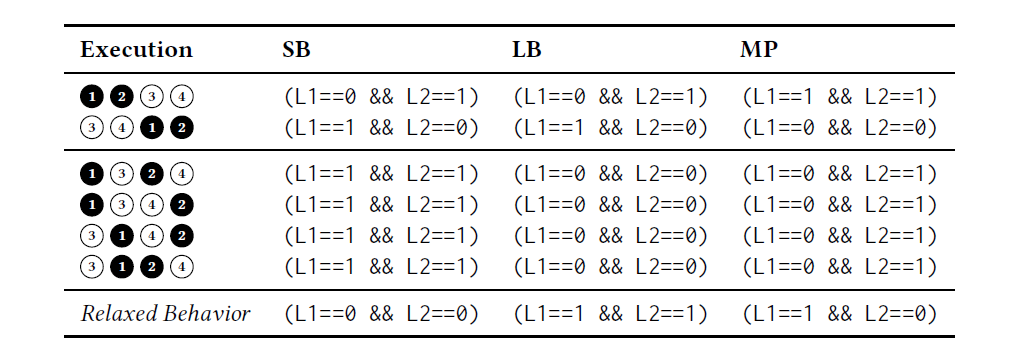
\includegraphics[scale=0.5]{SEQ-INT-RLX-EX.PNG}
            }
        \end{figure}

        %Add here the graphs from Figure 4
            %Point out the fact that Store Buffering is the least observed among all.
        \begin{figure}
            \makebox[\textwidth][c]{
                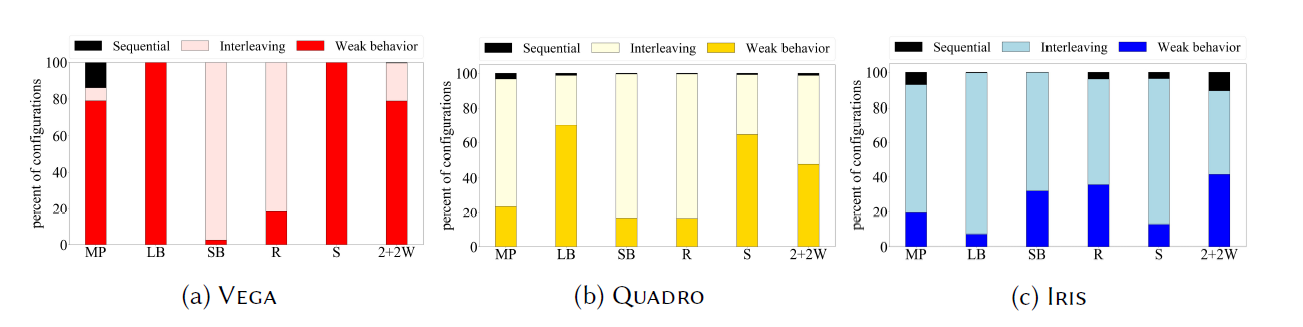
\includegraphics[scale=0.5]{SEQ-INT-RLX-OBS.PNG}
            }
        \end{figure}

    \end{frame}

    %Observation 2
    \begin{frame}{Rate of relaxed Behaviors observed w.r.t. Parameters}

        %Basically to check how much does each parameter, show relaxed behavior in runs done.
        %Take a parameter, run the program 10k times and then observe how many of them show relaxed behavior.
        %Note down the observations 


        %Add here Figure 5
        \begin{figure}
            \makebox[\textwidth][c]{
                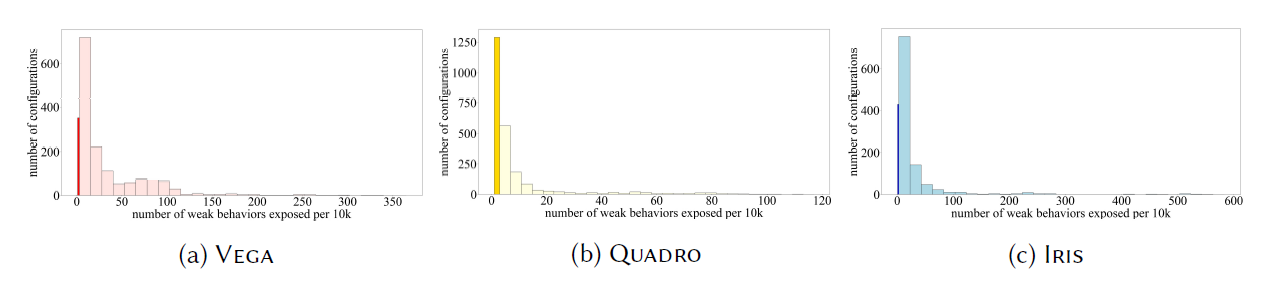
\includegraphics[scale=0.5]{RLX-OBS-RATE.PNG}
            }
        \end{figure}

        \begin{itemize}
            \item Note that the rate of decrease is exponential, indicating there are very few configurations showing more relaxed behaviors.
            \item This greatly influences the factor of reproducibility.
        \end{itemize}
        
    \end{frame}

    %Observation 3
    \begin{frame}{Stationary Relaxed Behaviors}

        \begin{itemize}
            \item Often relaxed behaviors will vary as the time passes by testing the same litmus test.
            \item This is due to external factors (heat/power consumption) that may influence the GPU/CPU to resort to other measures.
        \end{itemize}
        
        \begin{itemize}
            \item To check stationary factor of relaxed behaviors, choose a parameter and just keep running litmus tests based on it.
            \item See whether the same set of relaxed behaviors persist over time, with negligible variance. 
        \end{itemize}

        %Add here Figure 7, Poission and KS distribution graphs.
        \begin{figure}
            \makebox[\textwidth][c]{
                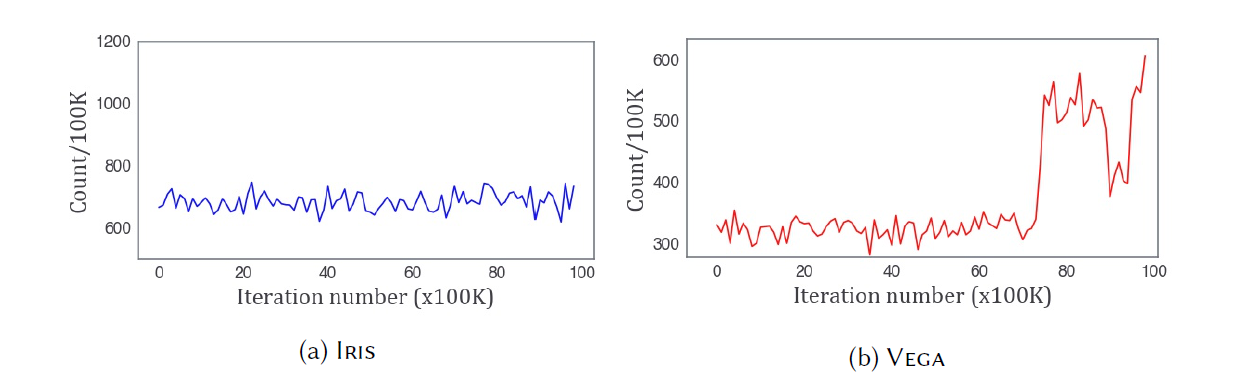
\includegraphics[scale=0.5]{GPU-STABLE-RLX.PNG}
            }
        \end{figure}

    \end{frame}

    %Observation 4 : Tuning Parameters
    \begin{frame}{Litmus Test Tuning (LTT)}

        %Explain what this means.
        \begin{itemize}
            \item Best litmus tests ? 
            \item How many relaxed behaviors a single litmus test proc? 
            \item Can a litmus test proc the same relaxed behaviors on different hardwares (if they allow it)? 
            \item For this, litmus test tuning is required.
        \end{itemize}
        
        Broadly three types of tuning
        \begin{itemize}
            \item Data peeking.
            \item Portable parameter testing.
            \item Cross correlations among litmus tests.
        \end{itemize}
        
    \end{frame}

    \note{Yes, we do observe a lot of relaxed behaviors with the above testing.
    However, it has not been checked whether the litmus tests used to force relaxed behaviors of different kinds the best one.
    Identifying the best ones relative to our requirements would greatly reduce the testing time and resource consumptions.
    Additionally, it could be that two litmus tests bring forth the same relaxed behavior, or that one brings about relaxed behavior from hardware that contains those behaviors brought by another.
    }

    \begin{frame}{LTT 1: Data Peeking}

        \begin{itemize}
            \item If in two tests, one clearly shows more promise of relaxed behaviors.
            \item The lesser promising can be discarded.
            \item This can save power and testing time. 
            \item Misc: Heat dissipation reduced.
        \end{itemize}

        \begin{figure}
            \makebox[\textwidth][c]{
                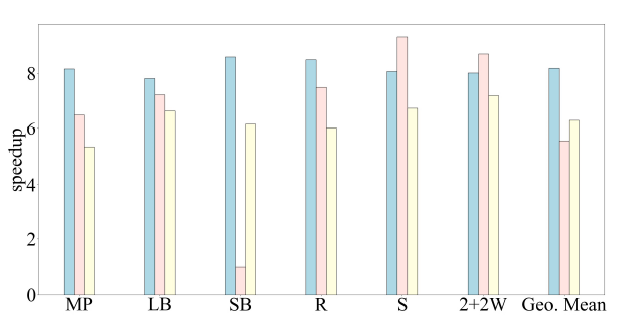
\includegraphics[scale=0.5]{DATA-PEEKING.PNG}
            }
        \end{figure}
        
    \end{frame}

    \note{
        It often becomes the case that one litmus test exhibit weak behaviors that contain that of another.
        If the former then on testing does show promise of showing all forms of weak behavior, it would be a wiser choice to discard the latter.
        However, this purely depends on our choice of testing. 
        It could be that we want one litmus test to represent just one weak behavior. 
        Thus, in that case it would be wiser to discard those that exhibit more than one weak behavior.
        The latter approach may be taken to enable better debugging problems in systems.
    }

    \begin{frame}{LTT 2: Portability based parameters}
        
        There are 3 ways we can divide our approach, assume we have N GPUs and M tests:
        \begin{itemize}
            \item Global - Across all GPUs, a single parameter which give most relaxed behaviors in all of them.
            \item Per-GPU - Each GPU will spur our representative parameter sets (N).
            \item Per-test - Each parameter per litmus test that works well for all GPUs (M).
            \item Per-GPU/test - For each GPU, each test, with best parameters (N * M). 
        \end{itemize}
        
        %TODO
    \end{frame}

    \note{Sometimes we might want to observe which parameter gives us the most relaxed behavior across all GPU/CPU.
    Such a parameter config will be beneficial for litmus testing across many devices.
    }

    \begin{frame}{LTT 3: Cross Test  Correlations}
        
        \begin{itemize}
            \item Two tests trigger the same behavior in question.
            \item Eg: $SB$ and $R$ will have read-after-write sequence, both of whose relaxed behavior will involve violating this order. 
            \item More beneficial to discard one case.
            \item Metric for this can be correlations matrix.
        \end{itemize}
        
        \begin{figure}
            \makebox[\textwidth][c]{
                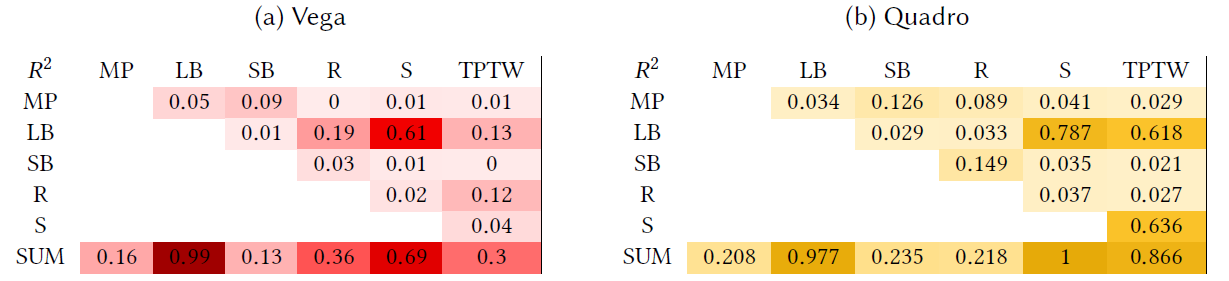
\includegraphics[scale=0.5]{CORR-MATRIX.PNG}
            }
        \end{figure}

    \end{frame}

    \note{Sometimes it may become the case that two tests (in our case litmus tests) trigger the same behavior that we are monitoring.
    In such a case, it would be beneficial to instead just use one of those test cases. 
    For this, we must have information that wrt the behavior how much the two tests are correlated.
    For example SB and R will have read-after-write sequence, both of whole relaxed behavior will involve this sequence.
    It would therefore be beneficial to use only one of them wrt the behavior of concern.
    }

    \begin{frame}{Conformance and Mutation Testing}

        \begin{itemize}
            \item Basically, we want to see what elements (semantics and hardware component wise) triggers the relaxed behaviors.
            \item Conformance testing using Minimal forbidden litmus tests (tests whose accesses, when relaxed even one of them will result in a relaxed behavior)
            \item The authors found a bug in Intel Iris doing this type of testing. 
            \item Mutation testing is using an implementation of the semantics and then creating a set where each element represents on implementation minus one semantic requirement. 
            \item The authors noted that the Nvdia GPU does not show many relaxed behaviors using mutation testing. 
        \end{itemize}
        

    \end{frame}

    \note{What this shows is that Nvdia memory model is relatively conservative wrt using relaxed semantics and one might need to relax or remove more than one semantic specification to let the GPU exhibit a high frequency of relaxed behaviors.
    Other forms of Conformance testing done was to check Multi-Copy or Non-Multi-Copy atomicity in hardware.}

    \begin{frame}{Conclusion}
        
        A more careful empirical testing of memory models (H/W) reveals to us several aspects of the system that play a role in relaxed behaviors:
        \begin{itemize}
            \item Different Hardware components may affect the testing results.
            \item Reproducibility, False Negatives and Redundancy.
            \item Stress on components not involved in the memory.
            \item Setting barriers, affinities towards threads of litmus tests.
            \item Litmus test tuning is helps reduce power consumption, heat dissipation, time and processing power.
            \item Tuning can also result in redundancy removal of litmus tests.
            \item Conformance testing reveals possible bugs in hardware(eg: Intel Iris).
            \item Mutation testing helps observe which hardware is more affinity for weak behaviors.
        \end{itemize}
        
        %We will need to actually take one lesson from each aspect of testing, make a list when finalizing the presentation.
    \end{frame}

    \begin{frame}{Thank you}
        Questions?
    \end{frame}

\end{document}